\documentclass[12pt, a4paper,twoside,titlepage]{article}
\usepackage[left=3cm,top=2cm,right=3cm,includehead]{geometry}

%% ¡¡ Modificar !! %%
\newcommand{\grado}{Grado en Ingeniería de la Ciberseguridad}
\newcommand{\pregunta} {Práctica 2: Representación de los datos}
\newcommand{\asignatura}{Metodologías de Desarrollo Seguro}
\newcommand{\curso}{Curso 2021-2022}
\newcommand{\autorA}{Alejandro Gallego Sánchez}
\newcommand{\autorB}{Adriano Campos Soto}
\newcommand{\autorC}{Ismael Gómez Esquilichi}
%% ¡¡ Modificar !! %%

\usepackage[round]{natbib}
\let\cite\citep

%%%%%%%%%%%%%%%%%%%%%%% Paquetes (no modificar)
\usepackage[utf8]{inputenc}
\usepackage[spanish,es-lcroman,es-tabla]{babel}
\usepackage[T1]{fontenc}
\usepackage[pdftex]{graphicx}
\usepackage{mathtools}
\usepackage{mathptmx}
\usepackage{amsmath}
\usepackage{amssymb}
\usepackage{enumitem}
\usepackage{minted}
\usepackage{caption}
\usepackage[justification=centering]{caption}
\setlength\abovecaptionskip{0.5em}
\setlength\belowcaptionskip{-0.25em}
 \usepackage[figuresright]{rotating}
 \usepackage{booktabs}
\usepackage{multirow}
\usepackage{xltabular}
\usepackage{longtable}
\usepackage{pdflscape}
\usepackage{afterpage}
\usepackage{relsize}
\usepackage{color}
\usepackage{xcolor}
\usepackage{booktabs}
\usepackage{subcaption}
\usepackage{amsmath}
\usepackage{minted}
\definecolor{linkcolor}{RGB}{52,59,144}
\definecolor{Comment}  {RGB}{169,082,044}
\definecolor{Bluedark} {RGB}{0,0,180}
\definecolor{Bluelight}{RGB}{070,100,250}
\definecolor{Browndark}{rgb}{0.2,0.2,0.2}
\definecolor{gray}{rgb}{0.6,0.6,0.6}
\usepackage{tikzpagenodes}
\usepackage[linesnumbered,ruled]{algorithm2e}
% \usepackage{algpseudocode}
\usepackage[hidelinks]{hyperref}
\usepackage{float}

%%%%%%%%%%%%%%%%%%%%%%% Estilo de código
\usepackage{textcomp}
\usepackage{bold-extra}
\usepackage{listings}
\usepackage{titlesec}
\usepackage{minted}
% Definition of \subparagraph emulating that of the standard classes
% \titleformat{\subparagraph}[runin]
%     {\normalfont\normalsize\bfseries}{\thesubparagraph}{1em}{}
% \titlespacing*{\subparagraph}{\parindent}{3.25ex plus 1ex minus .2ex}{1em}

% Definition of \subparagraph starting new line after heading
\titleformat{\subparagraph}
    {\normalfont\normalsize\bfseries}{\thesubparagraph}{1em}{}
\titlespacing*{\subparagraph}{\parindent}{3.25ex plus 1ex minus .2ex}{.75ex plus .1ex}
\newcommand{\code}{\lstinline[
  language={},
  columns=fullflexible,
  basicstyle=\color{Browndark}]
}
\lstdefinestyle{Default}{
  basicstyle = \relsize{-1}\ttfamily\color{Bluelight},
  keywordstyle=\color{Bluedark},
  stringstyle=\color{Browndark},
  commentstyle = \color{Comment},
  numberstyle=\tiny\color{Bluedark},
  xleftmargin=0.5cm,
  numbers=left,
  basewidth = 0.48em,
  columns=fullflexible,
  breaklines,
  breakatwhitespace=true,
  moredelim=*[s][\color{Browndark}]{[}{]},
  moredelim=[s][\color{Bluedark}]{\{}{\}},
  mathescape = true,
  upquote = true,
  inputencoding=utf8,
  extendedchars=true,
  showstringspaces=false,
  literate      =        % Support additional characters
  {á}{{\'a}}1  {é}{{\'e}}1  {í}{{\'i}}1 {ó}{{\'o}}1  {ú}{{\'u}}1
  {Á}{{\'A}}1  {É}{{\'E}}1  {Í}{{\'I}}1 {Ó}{{\'O}}1  {Ú}{{\'U}}1
  {ä}{{\"a}}1  {ë}{{\"e}}1  {ï}{{\"i}}1 {ö}{{\"o}}1  {ü}{{\"u}}1
  {ñ}{{\~n}}1  {Ñ}{{\~N}}1  {¿}{{?`}}1  {¡}{{!`}}1
  {\\\%}{{\textbackslash\%}}2  {~}{{\raisebox{0.5ex}{\texttildelow}}}1
  {<-}{{$\gets\ $}}1
}
\lstdefinestyle{Python}{style=Default, language=Python}
\lstdefinestyle{HTML}{style=Default, language=HTML}
\lstdefinestyle{Unity}{style=Default, language=[Sharp]C}
\lstdefinestyle{Latex}{style=Default, language=[LaTeX]TeX}
\lstdefinestyle{VHDL}{style=Default, language=VHDL}
%% Selecciona el estilo por defecto: Python, Unity, Latex, Default, ...
\lstset{style=VHDL}

%%%%%%%%%%%%%%%%%%%%%%% Estilo de páginas
\definecolor{mordantred19}{rgb}{0.68, 0.05, 0.0}
\usepackage{fancyhdr}
\pagestyle{fancy}
\fancyhf{}
\setlength{\headheight}{15.2pt}
%\renewcommand{\chaptermark}[1]{\markboth{\uppercase{#1}}{}}
\renewcommand*{\headrulewidth}{0pt}
%\fancyhead[EL]{ \textsf{\relsize{-1}{\grupo\ }} \hrulefill }
%\fancyhead[OR]{ \hrulefill \textsf{\relsize{-1}{\ \nouppercase\pregunta} } }
\fancyfoot[C]{\thepage}
\hypersetup{
    colorlinks=true,
    linkcolor=red,
    urlcolor=blue,
    citecolor=mordantred19,
    pdftitle={Práctica 2}
    }

%%%%%%%%%%%%%%%%%%%%%%%%%%%%%%% Portada
\renewcommand*{\maketitle}{%
\begin{titlepage}
  \pagestyle{plain}

  \begin{center}
    \vspace*{-4em}
    
\includegraphics[scale=.3]{Figuras/urjc.jpg}\\
    \vspace*{2em}
    \textsc{\LARGE Escuela Técnica Superior\\de Ingeniería Informática}\\
    \vspace*{2em}
    \textsc{\Large \grado}\\  
    \vspace*{\fill}
    \textbf{\LARGE \pregunta\\}  
    \vspace*{2em}
    \textsc{\large \asignatura\\}
    \vspace*{.5em}
    \textsc{\large \curso\\}  
    \vspace*{4em}\vspace*{\fill}
    \vspace*{4em}\vspace*{\fill}
    {%
      \large
      \begin{tabular}{rl}
        \textbf{Redactado por:} & \textbf{\autorA}\\
         & \textbf{\autorB}\\
         & \textbf{\autorC} \\
      \end{tabular}
    }
  \end{center}
  
\end{titlepage}
}

\sloppy

%%%%%%%%%%%%%%%%%%%%%%%%%%%%%%% Inicio del documento
\begin{document}

\maketitle

%%%% Inicio Artículo %%%%
\thispagestyle{empty}
\tableofcontents
\thispagestyle{empty}
\newpage
\setcounter{page}{1} % Comienza un contador de enumeración de las páginas.
\pagestyle{plain}

\section{Gráficos dinámicos}
Durante el desarrollo de la práctica se nos solicitaba cambiar los gráficos generados anteriormente de manera estática, por gráficos que se generasen de manera dinámica. Para ello hemos decidido utilizar la libreria \emph{plotly} para Python3. Esta librería permite generar gráficos dinámicos a partir de los \emph{dataframes} de la librería de \emph{pandas} para Python3 también. Además se han añadido una serie de modificadores que permitiesen establecer transformar los parámetros para obtener exactamente los gráficos que necesitábamos. 
\subsection{Top X usuarios críticos}
Durante este apartado de la práctica, se nos solicitaba el gráfico que obteníamos anteriormente el cual mostraba los usuarios más vulnerables de la página web. Este gráfico se genera apartir del siguiente método:
\begin{minted}{python}
    c, conn = connect_db("Entrega1/database/database.db")
    df1 = pd.read_sql_query("select * from users", conn)
    df1 = porcentaje_peligro(df1)
    df1 = usuarios_criticos(df1).head(x)
    data = plotlyF(df1, x)
\end{minted}
\begin{minted}{python}
def plotlyF(df: pd.DataFrame, x):
    trace = go.Bar(x=df["username"], y=df["porcentaje_click"])
    layout = go.Layout(title="Top %s usuarios críticos" % (x), xaxis=dict(title="username"),
                       yaxis=dict(title="porcentaje_click"))
    data = [trace]
    fig = go.Figure(data=data, layout=layout)
    fig_json = json.dumps(fig, cls=plotly.utils.PlotlyJSONEncoder)
    return fig_json
\end{minted}

Estas funciones permiten generar el gráfico que después mostramos a traves del template de \emph{jinja2}: 
\begin{minted}{html}

<div id='chart' class='chart'></div>
    <script src='https://cdn.plot.ly/plotly-latest.min.js'></script>
    <script type='text/javascript'>
        var graphs = {{data | safe}};
        Plotly.plot('chart',graphs,{});
    </script>

\end{minted}
Esto nos permite obtener el siguiente resultado:
\begin{figure}[H]
    \centering
    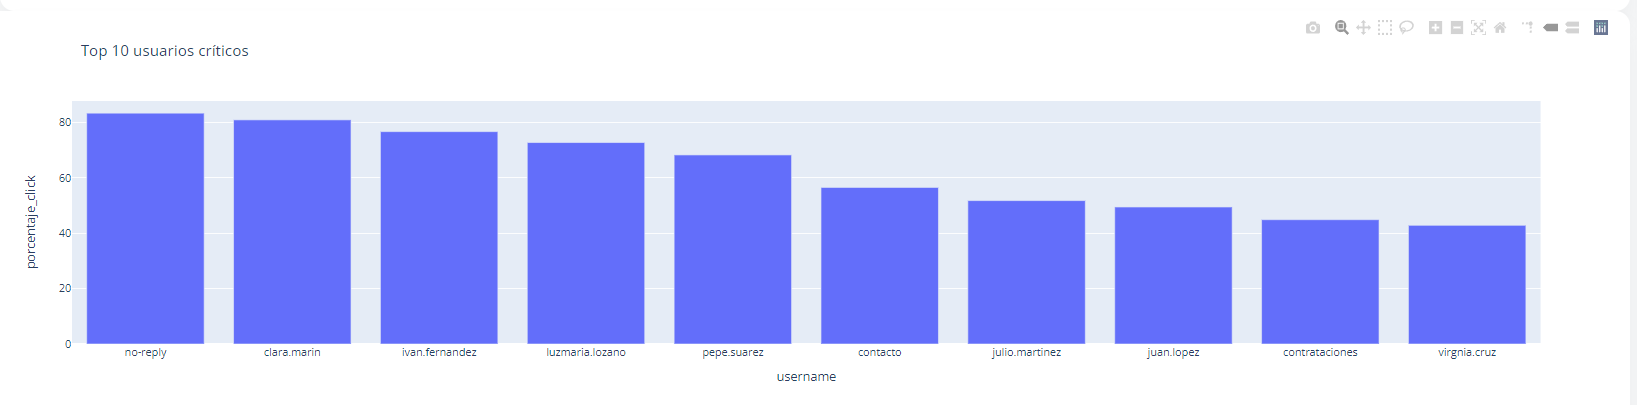
\includegraphics[width=1\linewidth]{Figuras/users-graph.png}
    \caption{Gráfico de usuarios generado con \emph{plotly}}
    \label{fig:graphusers}
\end{figure}
\subsection{Top X páginas webs vulnerables}
Este apartado es similar al anterior, con la salvedad de que esta vez se nos solicitaban sobre las webs vulnerables. Siguiendo con el procedimiento de \emph{plotly} hemos generado el gráfico de la siguiente manera:
\begin{minted}{python}
    c, conn = connect_db("Entrega1/database/database.db")
    dframe2 = pd.read_sql_query("SELECT * FROM legal", conn)
    dframe2 = get_paginas_desactualizadas(dframe2, limit=pages)
    print(dframe2)
    data2 = plotlyP(dframe2, pages)
\end{minted}
\begin{minted}{python}
def plotlyP(df: pd.DataFrame, x):
    trace = go.Bar(x=df["url"], y=df["n_politicas"])
    layout = go.Layout(title="Top %s webs vulnerables" % (x), xaxis=dict(title="web"),
                       yaxis=dict(title="porcentaje_click"))
    data = [trace]
    fig = go.Figure(data=data, layout=layout)
    fig_json = json.dumps(fig, cls=plotly.utils.PlotlyJSONEncoder)
    return fig_json
\end{minted}
Lo que insertado en la \emph{template} de \emph{jinja2} quedaría de la siguiente manera:
\begin{minted}{html}

<div id='chart2' class='chart'></div>
    <script src='https://cdn.plot.ly/plotly-latest.min.js'></script>
    <script type='text/javascript'>
        var graphs2 = {{data2 | safe}};
        Plotly.plot('chart2',graphs2,{});
    </script>

\end{minted}
Obteniendo el siguiente gráfico como resultado:
\begin{figure}[H]
    \centering
    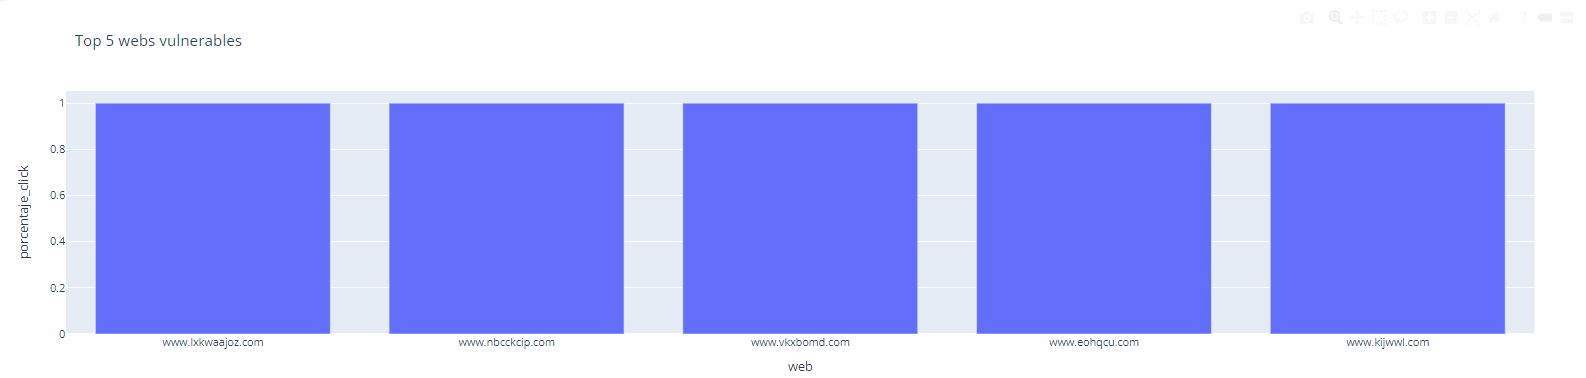
\includegraphics[width=1\linewidth]{Figuras/webs-graph.png}
    \caption{Gráfico de webs generado con \emph{plotly}}
    \label{fig:graphwebs}
\end{figure}
\section{Top X usuarios críticos filtrado}
Este apartado esta relacionado directamente con el anterior. Tendremos que tratar los \emph{dataframes} utilizados en el apartado 1.1 para poder obtener los valores que necesitemos. Para ello añadiremos otra función a nuestro servicio:
\begin{minted}{python}
def tratar_dataframe(df: pd.DataFrame, b: bool):
    if not b:
        df = df.loc[df['porcentaje_click'] < 50]
    else:
        df = df.loc[df['porcentaje_click'] >= 50]
    return df
\end{minted}
A la cual habrá que llamar antes de llamar a la función \emph{plotlyF()} de la siguiente manera:
\begin{minted}{python}
    c, conn = connect_db("Entrega1/database/database.db")
    df1 = pd.read_sql_query("select * from users", conn)
    df1 = porcentaje_peligro(df1)
    df1 = usuarios_criticos(df1)
    df1 = tratar_dataframe(df1, critico)
    data = plotlyF(df1.head(x), x)
\end{minted}
Los parámetros para generar los nuevos gráficos se pasan como variables \emph{GET} en la petición.

\section{Mostrar las últimas 10 vulnerabilidades a tiempo real}
Para el desarrollo de este apartado hemos usado la API de \url{https://cve.circl.lu/api/last} la cual nos permite obtener una lista con los últimos CVEs reportados y públicados. Hemos desarrollado una función que a traves de una petición \emph{GET} recogiese todas las vulnerabilidades y hemos formateado la respuesta para poder generar una lista con lo mismo. La función utilizada ha sido:
\begin{minted}{python}
def ejercicio4():
    r = requests.get("https://cve.circl.lu/api/last")
    jotason = json.loads(r.text)
    l = []
    for i in range(10):
        temp = jotason[i]
        l.append(temp)
    return l
\end{minted}
Luego hemos utilizado una librería de javascript, \emph{chartjs}, para poder mostrar los resultados devueltos en formato \emph{json} con un formato más amigable para el usuario. 
El resultado es el siguiente:
\begin{figure}[H]
    \centering
    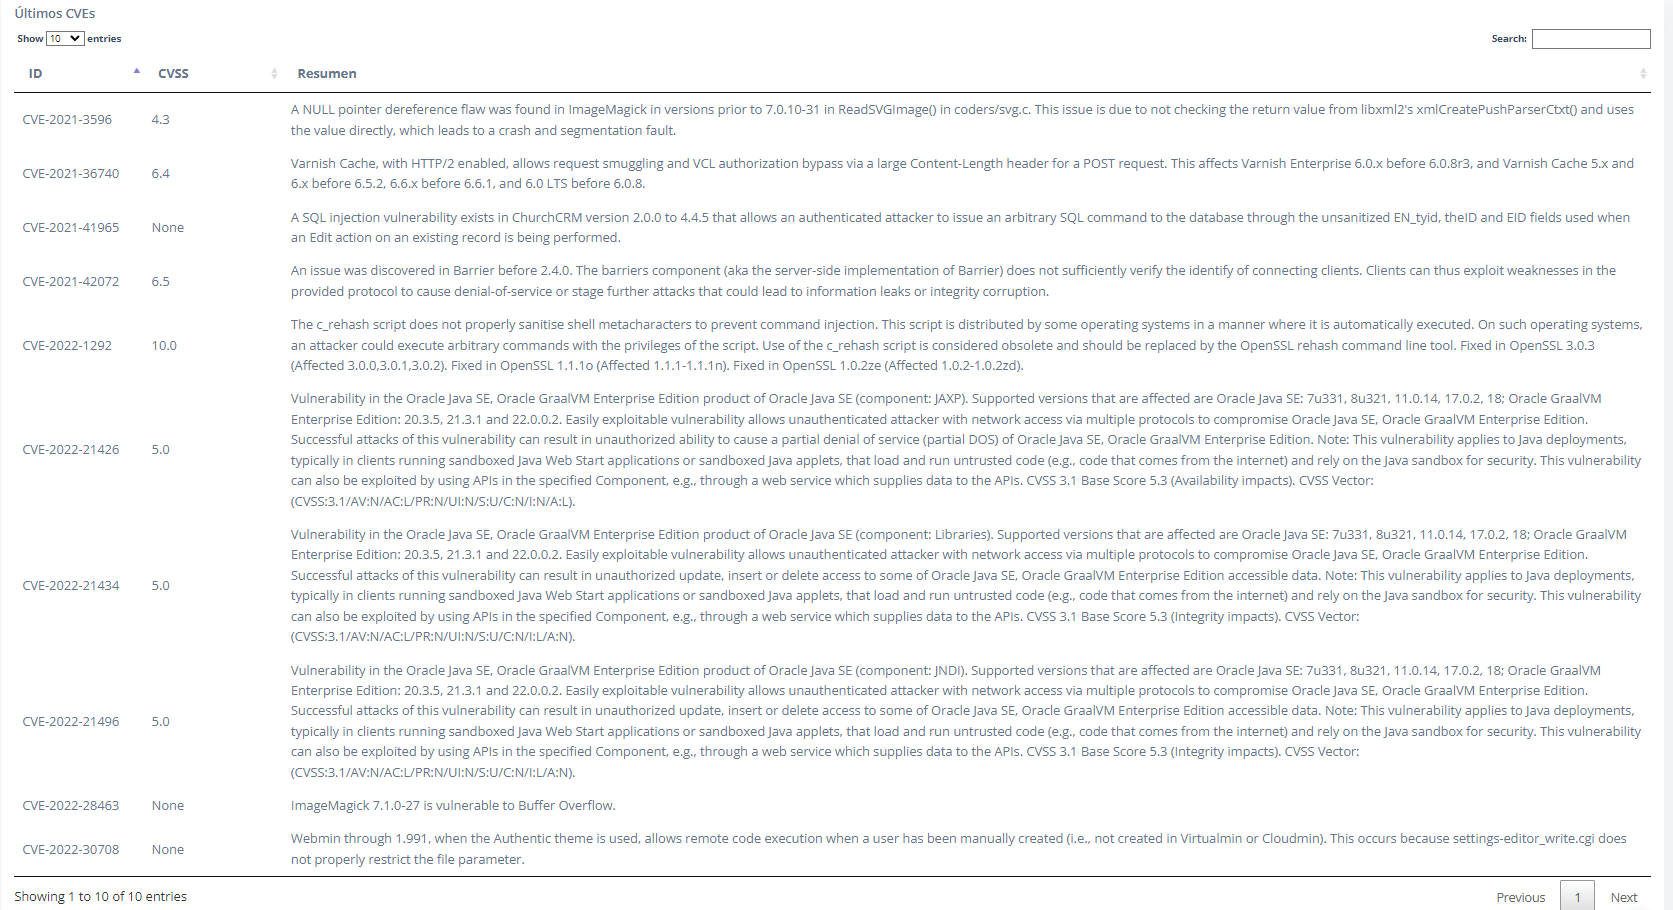
\includegraphics[width=1\linewidth]{Figuras/cve-list.png}
    \caption{Lista con los 10 últimos CVE}
    \label{fig:cvelist}
\end{figure}
\section{Nueva funcionalidad}
Como parte de la práctica se solicitaba implementar nueva funcionalidad al CMI, las opciones elegidas para este apartado han sido el sistema de login de usuarios, conexión con otra API en este caso \emph{exploitdb} y un modelo de \emph{machine learning} para poder predecir si un usuario será vulnerable o no.
\subsection{Sistema de login para usuarios}
Para implementar este modelo se ha tomado la decisión de continuar con el modelo de base de datos utilizado para la generación de los \emph{dataframes}, se ha utilizado una base de datos \emph{sqlite} y las funciones de Flask para poder crear sesiones. 
Se han implementado las funciones básicas de registro, login y logout. Ademas se ha impuesto que para poder acceder al dashboard el usuario tendría que estar \emph{loggeado} dentro de la propia aplicación. También se han añadido los endpoints y el html necesario para poder generar ambas vistas. Las funciones propias de este apartado son:
\begin{minted}{python}
@app.route('/register', methods=['GET', 'POST'])
def register_page():
    if request.method == 'GET':
        return render_template('pages/sign-up.html')
    elif request.method == 'POST':
        user = request.form['username']
        password = request.form['password']
        try:
            register_user(user, password)
            return redirect(url_for('login_page'))
        except sqlite3.IntegrityError as e:
            return render_template('pages/sign-up.html', error="""Ya existe 
            ese nombre de usuario""")
        except Exception as e:
            print(e)
            return redirect(url_for('register_page'))


@app.route('/login', methods=['GET', 'POST'])
def login_page():
    if request.method == 'GET':
        return render_template('pages/sign-in.html')
    else:
        user = request.form['user']
        passwd = request.form['password']
        log = login_user(user, passwd)
        if log == True:
            session['user'] = (user)
            return redirect(url_for('dashboard'))
        else:
            return render_template('pages/sign-in.html', error="""Credenciales 
            no validos, registrate""")


@app.route('/logout')
def log_out():
    if 'user' in session:
        session.pop('user')
    return redirect(url_for('login_page'))
\end{minted}


Y respecto a las funciones propias de \emph{SQL} las mismas serían:
\begin{minted}{python}
def register_user(username: str, password: str):
    try:
        cursor.execute("""INSERT INTO users_flaskitos(username, passwordHash)
            VALUES (?, ?)""",
                       (sqlescape(username), sqlescape(hash_password(password))))
    except sqlite3.IntegrityError as pr:
        raise
    con.commit()

def login_user(username: str, password: str):
    com = cursor.execute("""SELECT username, passwordHash FROM users_flaskitos
        WHERE username=(?)""",
                         [sqlescape(username)])
    res = com.fetchall()
    if len(res) == 1:
        if res[0][1] == hash_password(password):
            return True
        else:
            return False
    elif len(res) == 0:
        return "No existe"  # Cambiar a excepcion
    else:
        return "No te portes mal"
\end{minted}
Esto nos permite desarrollar toda la lógica de las sesiones de ususario mediante la propiedad \emph{session} de Flask, esta solo necesita añadirse y se encarga de gestionar los tokens necesarios en el cliente. Para autenticar a un cliente solo necesitamos esta linea:
\begin{minted}{python}
session['user'] = (user)
\end{minted}
\subsection{API \emph{exploitdb}}
Como segunda funcionalidad hemos decidido implementar una lista que contuviese los últimos exploits publicados en la famosa plataforma \emph{exploitdb}. Para ello hemos utilizado su propia API, la cual incluye un endpoint que devuelve los datos en formato XML \url{https://www.exploit-db.com/rss.xml}. Para recoger los resultados y poder tramitarlos a nuestra librería de javascript hemos implementado la siguiente función:
\begin{minted}{python}
def exploitdb():
    exploitdb_list = []
    last_exploitdb = feedparser.parse("https://www.exploit-db.com/rss.xml")
    for article in last_exploitdb.entries:
        name = article.description
        link = article.link
        category = article.title.split("]")[0][1:]
        exploitdb_list.append({"name": name, "category": category,
        "link": link, "saved": False})
    return exploitdb_list
\end{minted}
Y de nuevo hemos usado \emph{chartjs} para mostrarlo en nuestro HTML, obteniendo este resultado:
\begin{figure}[H]
    \centering
    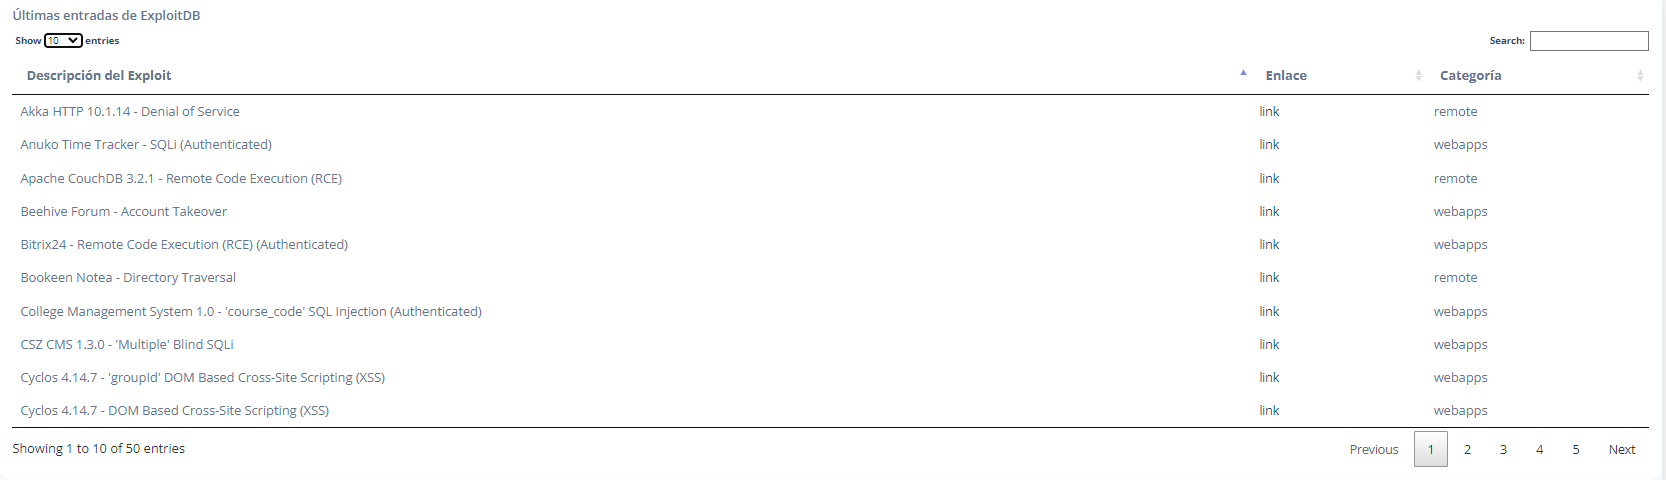
\includegraphics[width=1\linewidth]{Figuras/exploit-list.png}
    \caption{Lista con los últimos exploits de \emph{exploitdb}}
    \label{fig:exploitlist}
\end{figure}
\subsection{Modelo de predicción usuario crítico}
Hemos implementado un método en \emph{Flask} que recibe como parámetros el nombre de un usuarios, los correos de phishing que ha recibido y el número de ellos en los que ha hecho click.

Para construir el modelo, hemos usado los datos dados para hacer el apartado de \emph{machine learning}, en concreto hemos utilizado el algoritmo \emph{Random Forest} para el clasificador. Lo generamos con el siguiente código.

\begin{minted}{python}
@app.route('/iatraining', methods=['POST'])
def train_ai():
    if request.method == 'POST':
        name = request.form['nombre']
        erecibidos = int(request.form['erecibidos'])
        eclickados = int(request.form['eclickados'])
        if eclickados > erecibidos:
            return 'Error'
        x_train = datos.drop('vulnerable', axis=1)
        y_train = datos['vulnerable']

        rf_clf = RandomForestClassifier(max_depth=2, 
                    random_state=0, n_estimators=10)
        rf_clf.fit(x_train, y_train)

        predecir = pd.DataFrame({'emails_phishing_recibidos':
            [erecibidos], 'emails_phishing_clicados': [eclickados]})
        # Predict data on test part
        y_predict = rf_clf.predict(predecir)
        if y_predict[0] == 1:
            vuln = name + ' ES VULNERABLE'
        else:
            vuln = name + ' NO ES VULNERABLE'
        return vuln

\end{minted}

Este método recibe los parámetros necesarios para crear un \emph{dataframe} con los datos necesarios para predecir si el usuario dado es vulnerable o no lo es. Explicaremos más adelante como funciona internamente el algoritmo y el código que hemos utilizado para instanciar el clasificador. Si recibimos un \emph{1} el clasificador ha determinado que el usuario introducido es vulnerable. Si recibimos un \emph{0}, se ha clasificado como no vulnerable.

En la página web, esta feature se observa como en la figura \ref{IA}.

\begin{figure}[H]
    \centering
    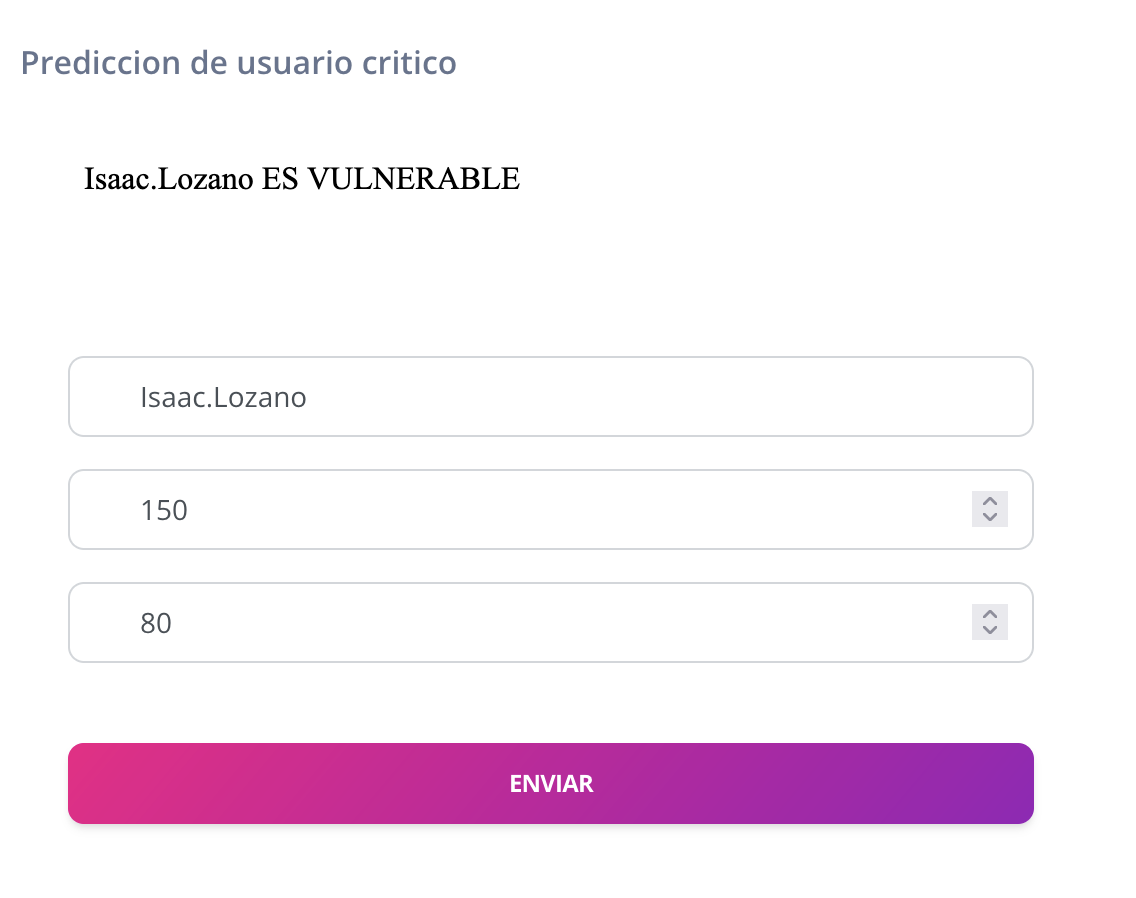
\includegraphics[width=1\linewidth]{Figuras/metodoia.png}
    \caption{UI creada para determinar por IA si un usuario es vulnerable o no}
    \label{fig:IA}
\end{figure}



\section{Machine Learning}
En esta práctica se nos facilitan dos ficheros \emph{json}. Uno de ellos es un pequeño dataset de usuarios que están etiquetados en función de si son vulnerables o no.
El otro fichero contiene otros usuarios con los mismos detalles pero no están etiquetados.
Hemos usado el primero para entrenar los algoritmos de los que vamos a hablar a continuación para intentar etiquetar los segundos.
\subsection{Decision Tree}
El algoritmo \emph{Decision Tree} es un algoritmo de aprendizaje supervisado que se usa para crear un modelo de árbol de decisiones a partir de un conjunto de datos de entrenamiento. El árbol de decisiones se puede usar para predecir el valor de una variable objetivo a partir de un conjunto de variables de entrada.
El código utilizado para generar el árbol y aplicarlo al conjunto de datos obtenido es el siguiente.

\begin{minted}{python}
    clf = tree.DecisionTreeClassifier()
    clf = clf.fit(x_train, y_train)

    y_predict = clf.predict(predecir)
    c = 0
    for i in y_predict:
        if i == 1:
            c += 1
    print("Decision Tree classified as vulnerable", str(c), "users")
\end{minted}
Se utiliza la librería \emph{sklearn} para instanciar un clasificador que utiliza el algoritmo \emph{Deicision Tree}, le pasamos los datos de entrenamiento para que genere un árbol de decisiones con las condiciones necesarias para etiquetar el conjunto de datos dato.
A continuación, le pasamos el conjunto de datos a predecir, y el método \emph{predict} devuelve una lista con etiquetas correspondientes a lo que ha dicho el árbol de cada usuario proporcionado.
El árbol generado se puede ver en la siguiente figura \ref{fig:DecisionTree}.
\begin{figure}[H]
    \centering
    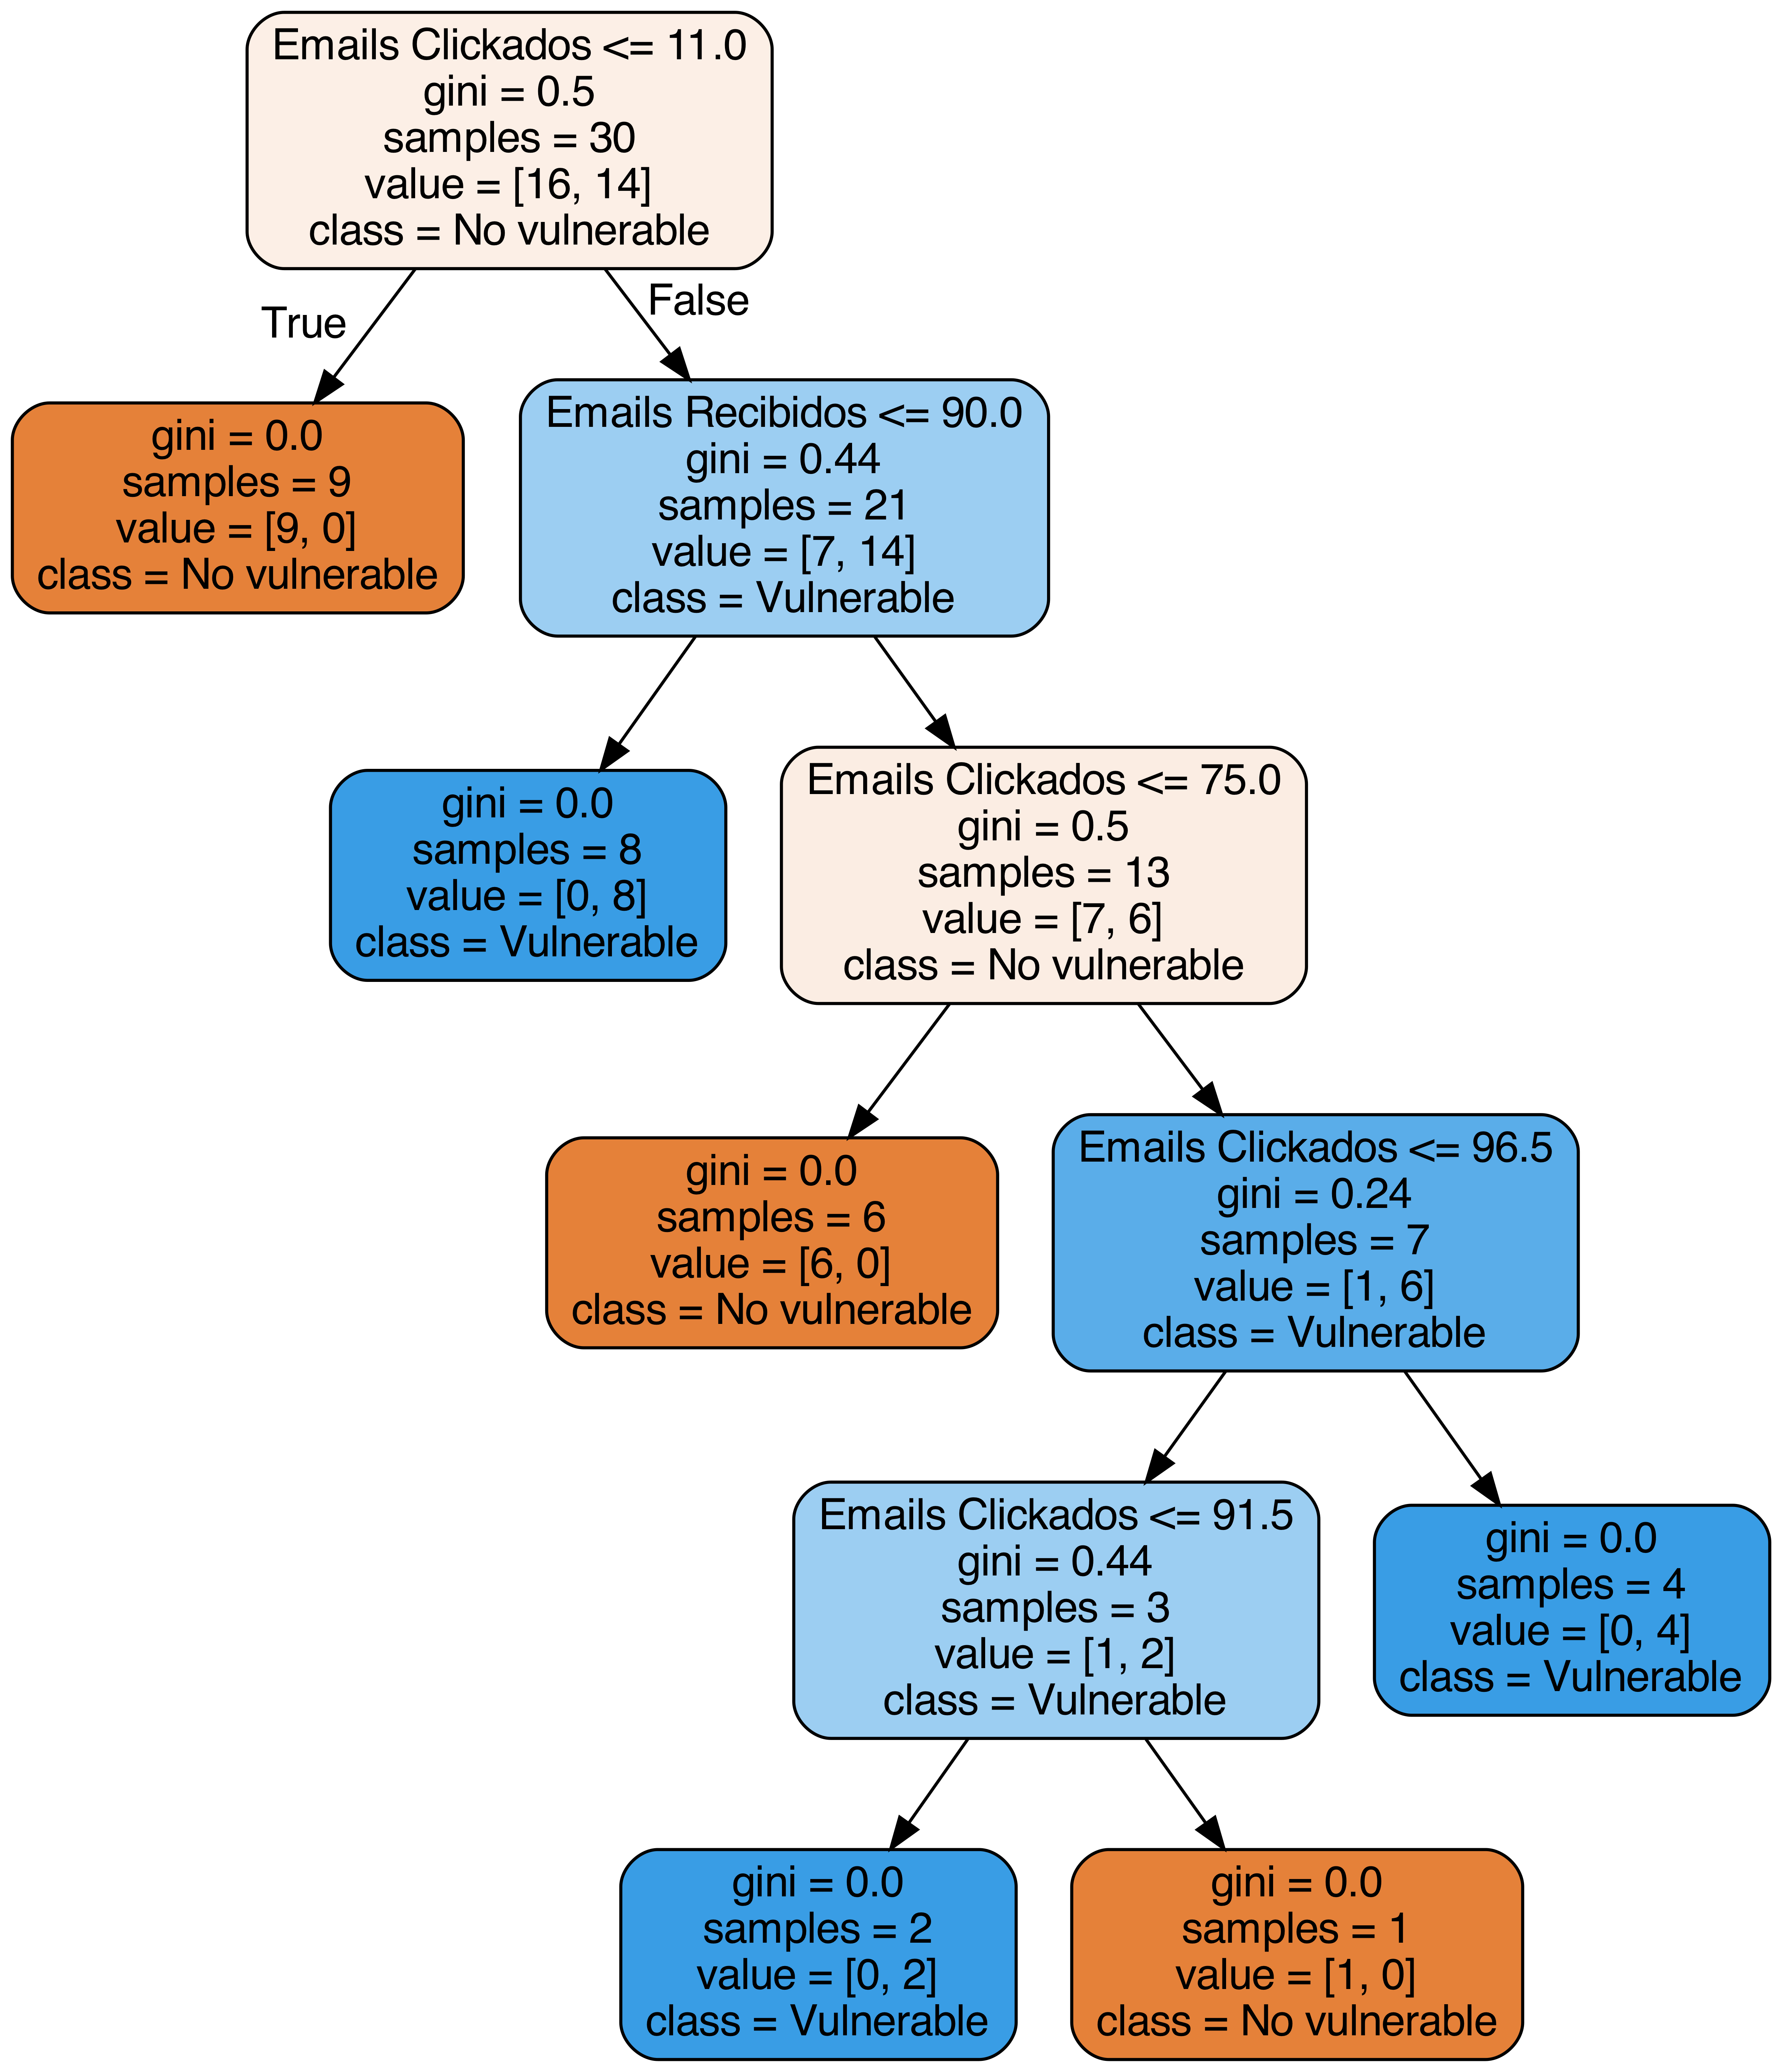
\includegraphics[width=70mm]{Figuras/decision_tree.png}
    \caption{Árbol de decisiones creado por el algoritmo}
    \label{fig:DecisionTree}
\end{figure}


\subsection{Random Forest}

El algoritmo de \emph{Random Forest} es un algoritmo de aprendizaje automático que se puede usar tanto para la regresión como para la clasificación. Su funcionamiento se basa en la creación de un número específico de árboles de decisión, generalmente se usan entre 10 y 100. Cada uno de los árboles en el bosque vota por el valor que predice para un determinado ejemplo, y el valor final que se asigna al ejemplo es la moda de los valores que votaron los árboles (es decir, el valor que más se repitió). 

La principal diferencia entre el algoritmo de \emph{Random Forest} y \emph{Decision Tree} es que el primero crea un número específico de árboles y luego selecciona el que mejor se ajusta, mientras que el segundo solo crea un árbol.

El siguiente código se encarga de crear los árboles de decisión basados en los datos de entrada e intenta etiquetar de forma adecuada los datos de predicción.
\begin{minted}{python}
    rf_clf = RandomForestClassifier(max_depth=2, random_state=0, n_estimators=10)
    rf_clf.fit(x_train, y_train)

    # Predict data on test part
    y_predict = rf_clf.predict(predecir)

    c = 0
    for i in y_predict:
        if i == 1:
            c += 1

    print("Random forest classified as vulnerable", str(c), "users")
\end{minted}

Primero se instancia el clasificador \emph{RandomForestClassifier} con varios parámetros, como la profundidad máxima de los árboles generados. En la siguiente figura se puede observar uno de los árboles generados por el algoritmo.

\begin{figure}[H]
    \centering
    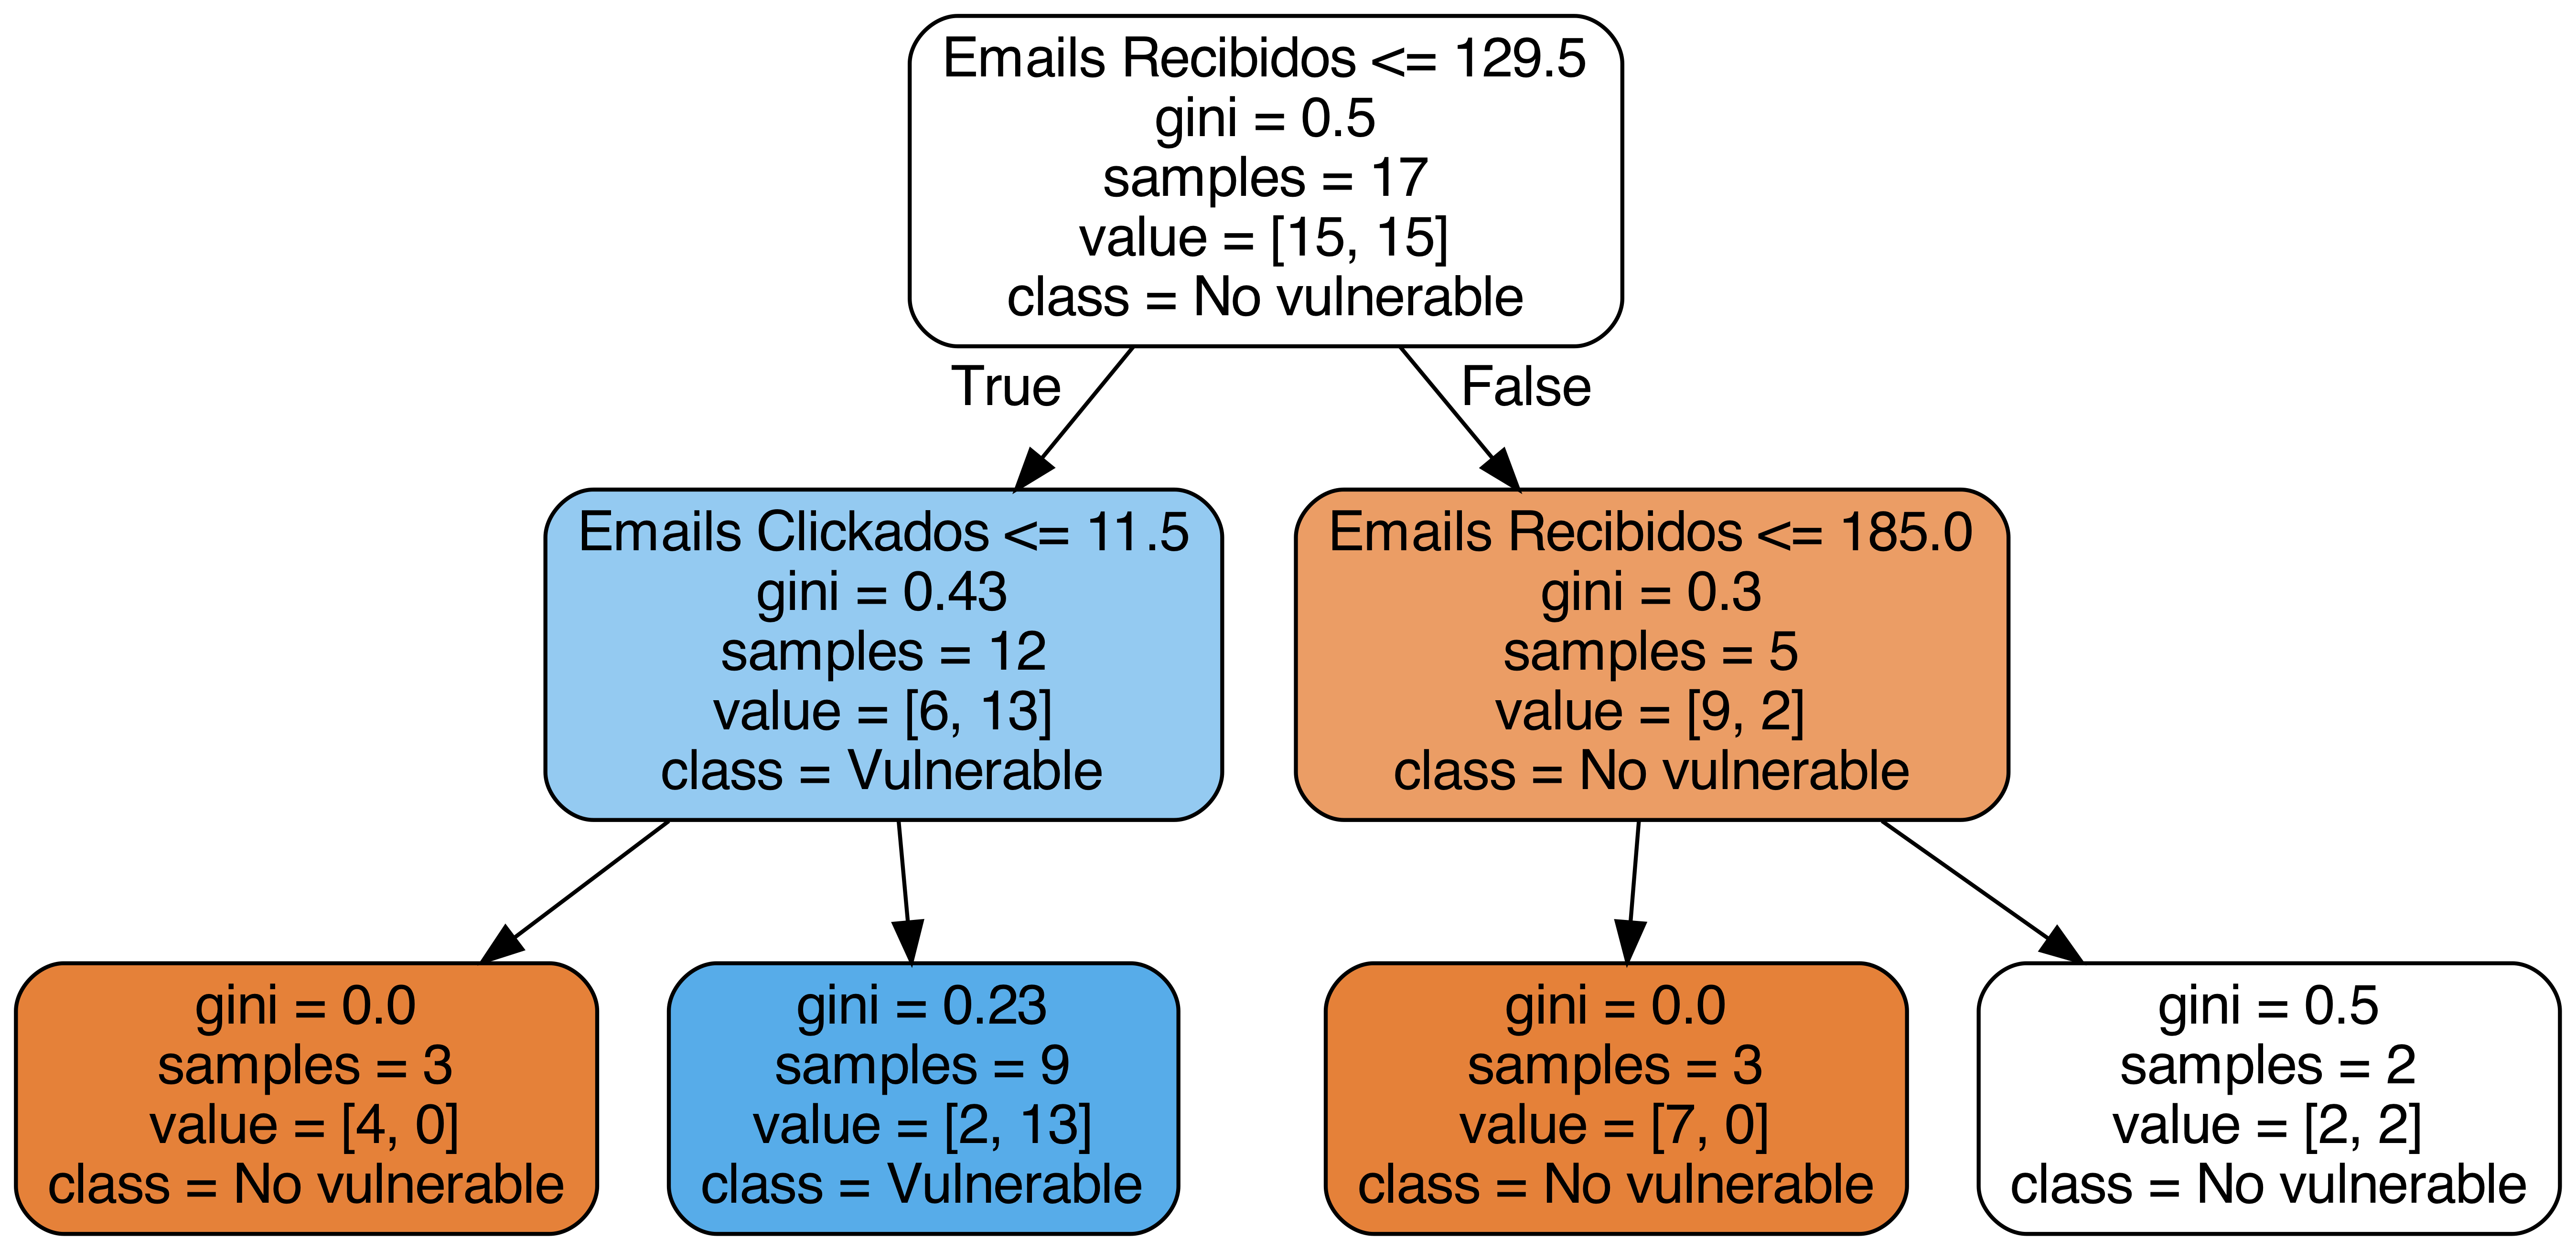
\includegraphics[width=1\linewidth]{Figuras/tree0.png}
    \caption{Árbol de decisiones creado por el algoritmo \emph{Random Forest}}
    \label{fig:RandomForest}
\end{figure}


\subsection{Regresión Linear}
El algoritmo de regresión linear es un método para predecir valores futuros en función de datos anteriores. Se basa en la idea de que existe una relación lineal entre los datos y, por lo tanto, podemos ajustar una línea a los datos para hacer predicciones.
\newline
Para realizar este ejercicio, hemos tenido que dividir el conjunto de información etiquetado en dos partes. El código sigue el modelo de los dos ejercicios anteriores. Lo que hacemos es instanciar la clase \emph{LinearRegression()}, ajustamos el modelo para los valores de entrenamiento en intentamos predecir los datos de valores no etiquetados.

\begin{minted}{python}
    data_x_train = data_x[:-20]
    data_x_test = data_x[-20:]
    data_y_train = data_y[:-20]
    data_y_test = data_y[-20:]
    regr = linear_model.LinearRegression()
    regr.fit(data_x_train, data_y_train)

    m = regr.coef_
    b = regr.intercept_
    x = data_x_test

    data_y_pred = regr.predict(np.array(data_x_test))
    for i in range(0, len(data_y_pred)):
        if data_y_pred[i] < 0.5:
            data_y_pred[i] = 0
        else:
            data_y_pred[i] = 1

    print(mean_squared_error(data_y_test, data_y_pred))
    print(accuracy_score(data_y_test, data_y_pred))

\end{minted}

La gráfica resultante se puede ver en la siguiente figura \ref{fig:LinearRegresion}.
\newpage
\begin{figure}[H]
    \centering
    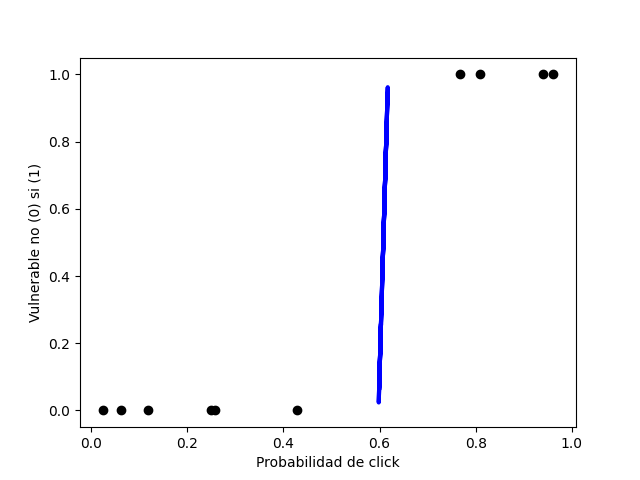
\includegraphics[width=1\linewidth]{Figuras/Figure_1.png}
    \caption{Gráfica generada por el algoritmo de regresión lineal}
    \label{fig:LinearRegresion}
\end{figure}


Como salida de los \emph{print()} obtenemos lo siguiente:
\begin{center}
Mean squared error: 0.35
Accuracy Regresión Lineal:  0.65
\end{center}


\end{document}